\documentclass{standalone}
\usepackage{tikz}
\usetikzlibrary{patterns, positioning}


\begin{document}
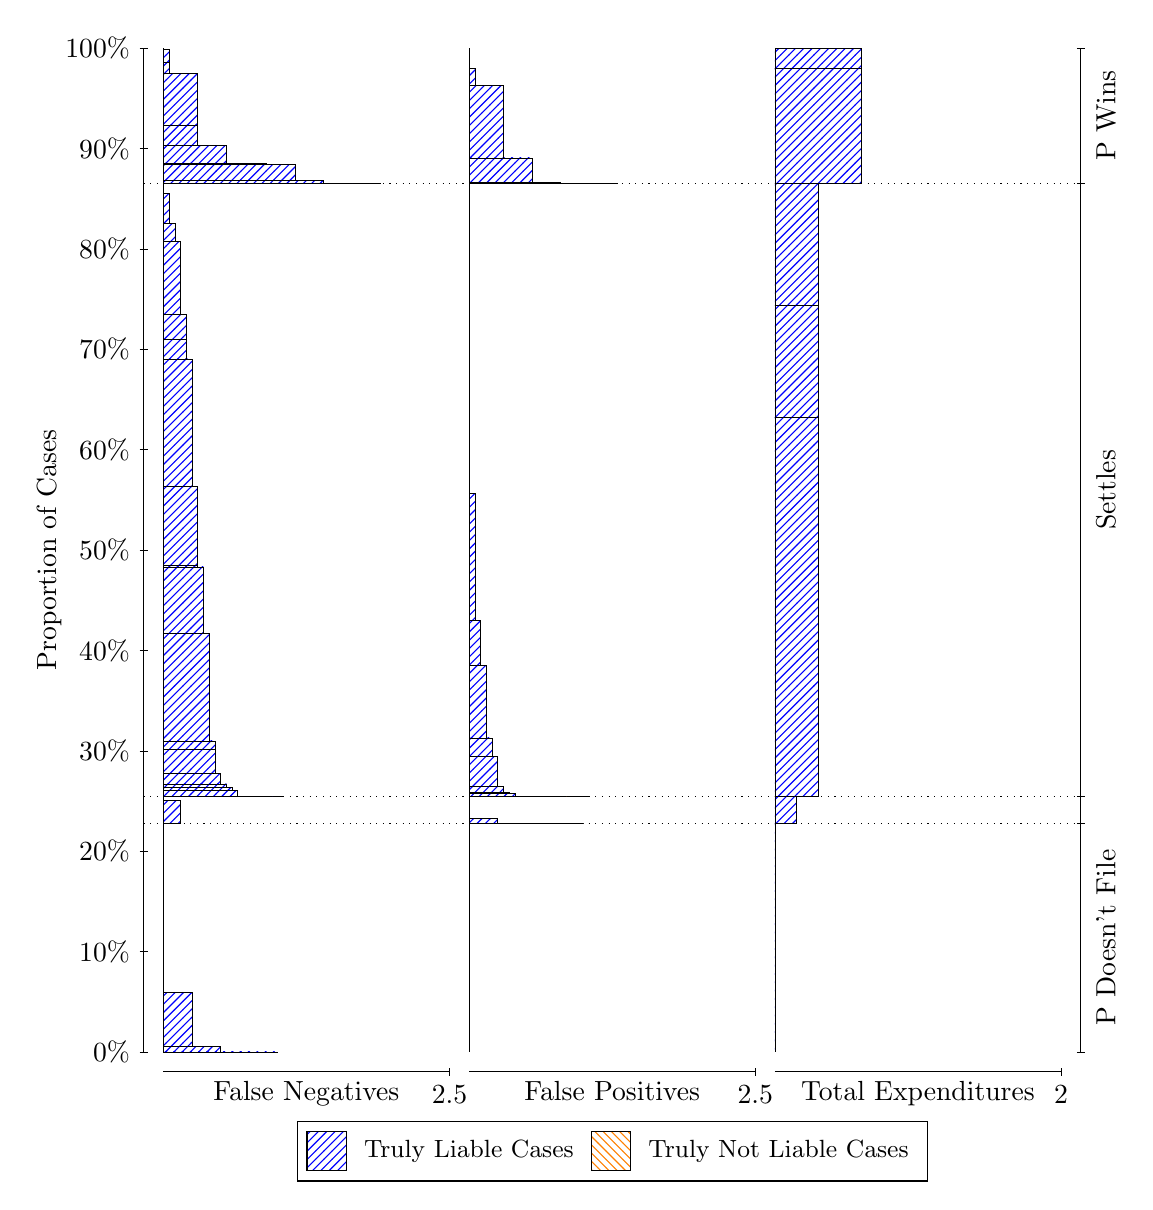
\begin{tikzpicture}
\draw[black, very thin] (1.5,1.75) -- (1.5,14.5);
\node[rotate=90, text=black, anchor=center] at (0.3, 8.125) {Proportion of Cases};
\draw[black, very thin] (1.45,1.75) -- (1.55,1.75);
\node[text=black, anchor=east] at (1.45, 1.75) {0\%};
\draw[black, very thin] (1.45,3.025) -- (1.55,3.025);
\node[text=black, anchor=east] at (1.45, 3.025) {10\%};
\draw[black, very thin] (1.45,4.3) -- (1.55,4.3);
\node[text=black, anchor=east] at (1.45, 4.3) {20\%};
\draw[black, very thin] (1.45,5.575) -- (1.55,5.575);
\node[text=black, anchor=east] at (1.45, 5.575) {30\%};
\draw[black, very thin] (1.45,6.85) -- (1.55,6.85);
\node[text=black, anchor=east] at (1.45, 6.85) {40\%};
\draw[black, very thin] (1.45,8.125) -- (1.55,8.125);
\node[text=black, anchor=east] at (1.45, 8.125) {50\%};
\draw[black, very thin] (1.45,9.4) -- (1.55,9.4);
\node[text=black, anchor=east] at (1.45, 9.4) {60\%};
\draw[black, very thin] (1.45,10.675) -- (1.55,10.675);
\node[text=black, anchor=east] at (1.45, 10.675) {70\%};
\draw[black, very thin] (1.45,11.95) -- (1.55,11.95);
\node[text=black, anchor=east] at (1.45, 11.95) {80\%};
\draw[black, very thin] (1.45,13.225) -- (1.55,13.225);
\node[text=black, anchor=east] at (1.45, 13.225) {90\%};
\draw[black, very thin] (1.45,14.5) -- (1.55,14.5);
\node[text=black, anchor=east] at (1.45, 14.5) {100\%};

\draw[black, very thin] (13.4,1.75) -- (13.4,14.5);
\draw[black, very thin] (13.35,1.75) -- (13.45,1.75);
\node[anchor=west] at (13.35, 1.75) {};
\draw[black, very thin] (13.35,4.6564) -- (13.45,4.6564);
\node[anchor=west] at (13.35, 4.6564) {};
\draw[black, very thin] (13.35,4.9964) -- (13.45,4.9964);
\node[anchor=west] at (13.35, 4.9964) {};
\draw[black, very thin] (13.35,12.782) -- (13.45,12.782);
\node[anchor=west] at (13.35, 12.782) {};
\draw[black, very thin] (13.35,14.5) -- (13.45,14.5);
\node[anchor=west] at (13.35, 14.5) {};

\draw[black, very thin, pattern color=blue, pattern=north east lines] (1.75,1.75) rectangle (3.2033,1.75);
\draw[black, very thin, pattern color=blue, pattern=north east lines] (1.75,1.75) rectangle (2.84,1.7506);
\draw[black, very thin, pattern color=blue, pattern=north east lines] (1.75,1.7506) rectangle (2.4767,1.8201);
\draw[black, very thin, pattern color=blue, pattern=north east lines] (1.75,1.8201) rectangle (2.1133,2.5087);
\draw[black, very thin, pattern color=orange, pattern=north west lines] (1.75,2.5087) rectangle (1.75,2.5087);
\draw[black, very thin, pattern color=blue, pattern=north east lines] (1.75,2.5087) rectangle (1.75,4.6564);
\draw[black, very thin, pattern color=blue, pattern=north east lines] (1.75,4.6564) rectangle (1.968,4.9408);
\draw[black, very thin, pattern color=orange, pattern=north west lines] (1.75,4.9408) rectangle (1.75,4.9408);
\draw[black, very thin, pattern color=blue, pattern=north east lines] (1.75,4.9408) rectangle (1.75,4.9964);
\draw[black, very thin, pattern color=blue, pattern=north east lines] (1.75,4.9964) rectangle (3.276,4.9964);
\draw[black, very thin, pattern color=blue, pattern=north east lines] (1.75,4.9964) rectangle (3.1307,4.9964);
\draw[black, very thin, pattern color=blue, pattern=north east lines] (1.75,4.9964) rectangle (2.9853,4.9964);
\draw[black, very thin, pattern color=blue, pattern=north east lines] (1.75,4.9964) rectangle (2.9127,4.9964);
\draw[black, very thin, pattern color=blue, pattern=north east lines] (1.75,4.9964) rectangle (2.84,4.9968);
\draw[black, very thin, pattern color=blue, pattern=north east lines] (1.75,4.9968) rectangle (2.7673,4.997);
\draw[black, very thin, pattern color=blue, pattern=north east lines] (1.75,4.997) rectangle (2.6947,5.0769);
\draw[black, very thin, pattern color=blue, pattern=north east lines] (1.75,5.0769) rectangle (2.622,5.1109);
\draw[black, very thin, pattern color=blue, pattern=north east lines] (1.75,5.1109) rectangle (2.5493,5.1535);
\draw[black, very thin, pattern color=blue, pattern=north east lines] (1.75,5.1535) rectangle (2.4767,5.2907);
\draw[black, very thin, pattern color=blue, pattern=north east lines] (1.75,5.2907) rectangle (2.404,5.5946);
\draw[black, very thin, pattern color=blue, pattern=north east lines] (1.75,5.5946) rectangle (2.404,5.7018);
\draw[black, very thin, pattern color=blue, pattern=north east lines] (1.75,5.7018) rectangle (2.3313,7.0665);
\draw[black, very thin, pattern color=blue, pattern=north east lines] (1.75,7.0665) rectangle (2.2587,7.9101);
\draw[black, very thin, pattern color=blue, pattern=north east lines] (1.75,7.9101) rectangle (2.186,7.933);
\draw[black, very thin, pattern color=blue, pattern=north east lines] (1.75,7.933) rectangle (2.186,8.9346);
\draw[black, very thin, pattern color=blue, pattern=north east lines] (1.75,8.9346) rectangle (2.1133,10.551);
\draw[black, very thin, pattern color=blue, pattern=north east lines] (1.75,10.551) rectangle (2.0407,10.797);
\draw[black, very thin, pattern color=blue, pattern=north east lines] (1.75,10.797) rectangle (2.0407,11.116);
\draw[black, very thin, pattern color=blue, pattern=north east lines] (1.75,11.116) rectangle (1.968,12.041);
\draw[black, very thin, pattern color=blue, pattern=north east lines] (1.75,12.041) rectangle (1.8953,12.272);
\draw[black, very thin, pattern color=blue, pattern=north east lines] (1.75,12.272) rectangle (1.8227,12.272);
\draw[black, very thin, pattern color=blue, pattern=north east lines] (1.75,12.272) rectangle (1.8227,12.653);
\draw[black, very thin, pattern color=orange, pattern=north west lines] (1.75,12.653) rectangle (1.75,12.653);
\draw[black, very thin, pattern color=blue, pattern=north east lines] (1.75,12.653) rectangle (1.75,12.782);
\draw[black, very thin, pattern color=blue, pattern=north east lines] (1.75,12.782) rectangle (4.5113,12.782);
\draw[black, very thin, pattern color=blue, pattern=north east lines] (1.75,12.782) rectangle (4.148,12.782);
\draw[black, very thin, pattern color=blue, pattern=north east lines] (1.75,12.782) rectangle (3.7847,12.818);
\draw[black, very thin, pattern color=blue, pattern=north east lines] (1.75,12.818) rectangle (3.4213,13.026);
\draw[black, very thin, pattern color=blue, pattern=north east lines] (1.75,13.026) rectangle (3.276,13.026);
\draw[black, very thin, pattern color=blue, pattern=north east lines] (1.75,13.026) rectangle (3.058,13.037);
\draw[black, very thin, pattern color=blue, pattern=north east lines] (1.75,13.037) rectangle (2.9127,13.037);
\draw[black, very thin, pattern color=blue, pattern=north east lines] (1.75,13.037) rectangle (2.6947,13.037);
\draw[black, very thin, pattern color=blue, pattern=north east lines] (1.75,13.037) rectangle (2.5493,13.259);
\draw[black, very thin, pattern color=blue, pattern=north east lines] (1.75,13.259) rectangle (2.3313,13.259);
\draw[black, very thin, pattern color=blue, pattern=north east lines] (1.75,13.259) rectangle (2.186,13.524);
\draw[black, very thin, pattern color=blue, pattern=north east lines] (1.75,13.524) rectangle (2.186,14.176);
\draw[black, very thin, pattern color=blue, pattern=north east lines] (1.75,14.176) rectangle (1.8227,14.32);
\draw[black, very thin, pattern color=blue, pattern=north east lines] (1.75,14.32) rectangle (1.8227,14.484);
\draw[black, very thin, pattern color=orange, pattern=north west lines] (1.75,14.484) rectangle (1.75,14.484);
\draw[black, very thin, pattern color=blue, pattern=north east lines] (1.75,14.484) rectangle (1.75,14.5);
\draw[black, very thin, pattern color=orange, pattern=north west lines] (5.6333,1.75) rectangle (5.6333,1.75);
\draw[black, very thin, pattern color=blue, pattern=north east lines] (5.6333,1.75) rectangle (5.6333,4.6564);
\draw[black, very thin, pattern color=orange, pattern=north west lines] (5.6333,4.6564) rectangle (7.0867,4.6564);
\draw[black, very thin, pattern color=blue, pattern=north east lines] (5.6333,4.6564) rectangle (7.0867,4.6564);
\draw[black, very thin, pattern color=blue, pattern=north east lines] (5.6333,4.6564) rectangle (6.7233,4.6564);
\draw[black, very thin, pattern color=blue, pattern=north east lines] (5.6333,4.6564) rectangle (6.36,4.6568);
\draw[black, very thin, pattern color=blue, pattern=north east lines] (5.6333,4.6568) rectangle (5.9967,4.712);
\draw[black, very thin, pattern color=blue, pattern=north east lines] (5.6333,4.712) rectangle (5.6333,4.9964);
\draw[black, very thin, pattern color=orange, pattern=north west lines] (5.6333,4.9964) rectangle (7.1593,4.9964);
\draw[black, very thin, pattern color=blue, pattern=north east lines] (5.6333,4.9964) rectangle (7.1593,4.9964);
\draw[black, very thin, pattern color=orange, pattern=north west lines] (5.6333,4.9964) rectangle (6.8687,4.9964);
\draw[black, very thin, pattern color=blue, pattern=north east lines] (5.6333,4.9964) rectangle (6.8687,4.9964);
\draw[black, very thin, pattern color=blue, pattern=north east lines] (5.6333,4.9964) rectangle (6.796,4.9964);
\draw[black, very thin, pattern color=orange, pattern=north west lines] (5.6333,4.9964) rectangle (6.7233,4.9964);
\draw[black, very thin, pattern color=blue, pattern=north east lines] (5.6333,4.9964) rectangle (6.7233,4.9964);
\draw[black, very thin, pattern color=orange, pattern=north west lines] (5.6333,4.9964) rectangle (6.578,4.9964);
\draw[black, very thin, pattern color=blue, pattern=north east lines] (5.6333,4.9964) rectangle (6.578,4.9964);
\draw[black, very thin, pattern color=blue, pattern=north east lines] (5.6333,4.9964) rectangle (6.5053,4.9964);
\draw[black, very thin, pattern color=orange, pattern=north west lines] (5.6333,4.9964) rectangle (6.4327,4.9964);
\draw[black, very thin, pattern color=blue, pattern=north east lines] (5.6333,4.9964) rectangle (6.4327,4.9965);
\draw[black, very thin, pattern color=blue, pattern=north east lines] (5.6333,4.9965) rectangle (6.36,4.9965);
\draw[black, very thin, pattern color=orange, pattern=north west lines] (5.6333,4.9965) rectangle (6.2873,4.9965);
\draw[black, very thin, pattern color=blue, pattern=north east lines] (5.6333,4.9965) rectangle (6.2873,4.997);
\draw[black, very thin, pattern color=blue, pattern=north east lines] (5.6333,4.997) rectangle (6.2147,5.0292);
\draw[black, very thin, pattern color=orange, pattern=north west lines] (5.6333,5.0292) rectangle (6.142,5.0292);
\draw[black, very thin, pattern color=blue, pattern=north east lines] (5.6333,5.0292) rectangle (6.142,5.0478);
\draw[black, very thin, pattern color=blue, pattern=north east lines] (5.6333,5.0478) rectangle (6.0693,5.125);
\draw[black, very thin, pattern color=orange, pattern=north west lines] (5.6333,5.125) rectangle (5.9967,5.125);
\draw[black, very thin, pattern color=blue, pattern=north east lines] (5.6333,5.125) rectangle (5.9967,5.5067);
\draw[black, very thin, pattern color=blue, pattern=north east lines] (5.6333,5.5067) rectangle (5.924,5.7375);
\draw[black, very thin, pattern color=blue, pattern=north east lines] (5.6333,5.7375) rectangle (5.8513,6.662);
\draw[black, very thin, pattern color=blue, pattern=north east lines] (5.6333,6.662) rectangle (5.7787,7.2272);
\draw[black, very thin, pattern color=blue, pattern=north east lines] (5.6333,7.2272) rectangle (5.706,8.8437);
\draw[black, very thin, pattern color=blue, pattern=north east lines] (5.6333,8.8437) rectangle (5.6333,12.782);
\draw[black, very thin, pattern color=orange, pattern=north west lines] (5.6333,12.782) rectangle (7.5227,12.782);
\draw[black, very thin, pattern color=blue, pattern=north east lines] (5.6333,12.782) rectangle (7.5227,12.782);
\draw[black, very thin, pattern color=orange, pattern=north west lines] (5.6333,12.782) rectangle (7.1593,12.782);
\draw[black, very thin, pattern color=blue, pattern=north east lines] (5.6333,12.782) rectangle (7.1593,12.782);
\draw[black, very thin, pattern color=orange, pattern=north west lines] (5.6333,12.782) rectangle (6.796,12.782);
\draw[black, very thin, pattern color=blue, pattern=north east lines] (5.6333,12.782) rectangle (6.796,12.798);
\draw[black, very thin, pattern color=orange, pattern=north west lines] (5.6333,12.798) rectangle (6.4327,12.798);
\draw[black, very thin, pattern color=blue, pattern=north east lines] (5.6333,12.798) rectangle (6.4327,13.106);
\draw[black, very thin, pattern color=blue, pattern=north east lines] (5.6333,13.106) rectangle (6.0693,14.023);
\draw[black, very thin, pattern color=orange, pattern=north west lines] (5.6333,14.023) rectangle (5.924,14.023);
\draw[black, very thin, pattern color=blue, pattern=north east lines] (5.6333,14.023) rectangle (5.924,14.023);
\draw[black, very thin, pattern color=blue, pattern=north east lines] (5.6333,14.023) rectangle (5.706,14.245);
\draw[black, very thin, pattern color=orange, pattern=north west lines] (5.6333,14.245) rectangle (5.6333,14.245);
\draw[black, very thin, pattern color=blue, pattern=north east lines] (5.6333,14.245) rectangle (5.6333,14.5);
\draw[black, very thin, pattern color=orange, pattern=north west lines] (9.5167,1.75) rectangle (9.5167,1.75);
\draw[black, very thin, pattern color=blue, pattern=north east lines] (9.5167,1.75) rectangle (9.5167,4.6564);
\draw[black, very thin, pattern color=orange, pattern=north west lines] (9.5167,4.6564) rectangle (9.7892,4.6564);
\draw[black, very thin, pattern color=blue, pattern=north east lines] (9.5167,4.6564) rectangle (9.7892,4.9964);
\draw[black, very thin, pattern color=orange, pattern=north west lines] (9.5167,4.9964) rectangle (10.062,4.9964);
\draw[black, very thin, pattern color=blue, pattern=north east lines] (9.5167,4.9964) rectangle (10.062,9.8057);
\draw[black, very thin, pattern color=orange, pattern=north west lines] (9.5167,9.8057) rectangle (10.062,9.8057);
\draw[black, very thin, pattern color=blue, pattern=north east lines] (9.5167,9.8057) rectangle (10.062,11.23);
\draw[black, very thin, pattern color=orange, pattern=north west lines] (9.5167,11.23) rectangle (10.062,11.23);
\draw[black, very thin, pattern color=blue, pattern=north east lines] (9.5167,11.23) rectangle (10.062,12.782);
\draw[black, very thin, pattern color=orange, pattern=north west lines] (9.5167,12.782) rectangle (10.607,12.782);
\draw[black, very thin, pattern color=blue, pattern=north east lines] (9.5167,12.782) rectangle (10.607,14.245);
\draw[black, very thin, pattern color=orange, pattern=north west lines] (9.5167,14.245) rectangle (10.607,14.245);
\draw[black, very thin, pattern color=blue, pattern=north east lines] (9.5167,14.245) rectangle (10.607,14.5);
\draw[black, dotted] (1.5,4.6564) -- (13.4,4.6564);
\draw[black, dotted] (1.5,4.9964) -- (13.4,4.9964);
\draw[black, dotted] (1.5,12.782) -- (13.4,12.782);
\draw[black, very thin] (1.75,1.5) -- (5.3833,1.5);
\node[text=black, anchor=north] at (3.5667, 1.5) {False Negatives};
\draw[black, very thin] (5.3833,1.45) -- (5.3833,1.55);
\node[text=black, anchor=north] at (5.3833, 1.45) {2.5};

\draw[black, very thin] (5.6333,1.5) -- (9.2667,1.5);
\node[text=black, anchor=north] at (7.45, 1.5) {False Positives};
\draw[black, very thin] (9.2667,1.45) -- (9.2667,1.55);
\node[text=black, anchor=north] at (9.2667, 1.45) {2.5};

\draw[black, very thin] (9.5167,1.5) -- (13.15,1.5);
\node[text=black, anchor=north] at (11.333, 1.5) {Total Expenditures};
\draw[black, very thin] (13.15,1.45) -- (13.15,1.55);
\node[text=black, anchor=north] at (13.15, 1.45) {2};

\node[text=black, centered, rotate=90] at (13.72, 3.2032) {P Doesn't File};

\node[text=black, centered, rotate=90] at (13.72, 8.8891) {Settles};
\node[text=black, centered, rotate=90] at (13.72, 13.641) {P Wins};

\draw (7.449999999999999,1.5) node[draw=none] (baseCoordinate) {};
\begin{scope}[align=center]
        \matrix[scale=0.5, draw=black, below=0.5cm of baseCoordinate, nodes={draw}, column sep=0.1cm]{
            \node[rectangle, draw, minimum width=0.5cm, minimum height=0.5cm, pattern color=blue, pattern=north east lines] {}; &
            \node[draw=none, font=\small, text=black] (B) {Truly Liable Cases}; &
            \node[rectangle, draw, minimum width=0.5cm, minimum height=0.5cm, pattern color=orange, pattern=north west lines] {}; &
            \node[draw=none, font=\small, text=black] (B) {Truly Not Liable Cases}; \\
            };
\end{scope}

\end{tikzpicture}
\end{document}